% Copyright 2026 Sreeram Anil
% SPDX-License-Identifier: CC-BY-4.0
\chapter{Attitude-estimation results}
\label{ch:res-attitude}

\section{Why an attitude benchmark is in a battery report}

The attitude problem is in this library for two reasons. It is the problem on which most of
the estimators of Parts~III--V were first flown --- the multiplicative EKF, the complementary
filter and the single-frame solutions of Wahba's problem are the aerospace heritage of the
Kalman-type filters that the battery chapters apply --- and it is the second concrete model
that the model-agnostic interface of \cref{ch:library} was tested against: a state on the
rotation group with a gyro-bias augmentation, three-axis vector measurements and a
\SI{100}{\hertz} rate, none of which the battery model exercises. The nine estimators of
Part~XIII run on the synthetic flight of \cref{sec:ds-imu} --- take-off, climb, three
\SI{60}{\second} coordinated turns at \ang{25} of bank, cruise, descent and final --- with a
consumer-grade inertial unit, a calibrated but not perfect compass (a residual hard-iron offset
of \SI{0.42}{\micro\tesla}, \SI{0.87}{\percent} of the field), and six scenarios: nominal, a
\ang{46} initial error, a \SI{3}{\degree\per\second} gyro bias, a \SI{25}{\micro\tesla} magnetic
disturbance, vibration, and a high-dynamics variant. \Cref{tab:imu_overview} gives the mission
RMS attitude error (\cref{eq:ds-imu-angdist}) and \cref{fig:res-imu} the same numbers by
scenario.

% Copyright 2026 Sreeram Anil
% SPDX-License-Identifier: CC-BY-4.0
\begin{table}[H]\centering\footnotesize\setlength{\tabcolsep}{3pt}\caption{Attitude estimators: RMS attitude error [deg] by scenario (mean over seeds) and cost per 100\,Hz sample.}\label{tab:imu_overview}
\begin{tabular}{lrrrrrrrr}\toprule estimator & \rotatebox{60}{nominal} & \rotatebox{60}{init\_error} & \rotatebox{60}{gyro\_bias} & \rotatebox{60}{mag\_disturbance} & \rotatebox{60}{vibration} & \rotatebox{60}{high\_dynamics} & ns/step & bytes \\ \midrule
Complementary & 6.57 & 6.79 & 17.58 & 6.71 & 6.58 & 6.58 & 362 & 272 \\
Madgwick & 17.60 & 17.74 & 17.62 & 19.01 & 14.78 & 18.43 & 112 & 272 \\
Madgwick-Gated & 5.78 & 6.17 & 5.79 & 5.78 & 3.22 & 5.34 & 138 & 272 \\
Mahony & 18.40 & 18.51 & 18.44 & 20.41 & 18.28 & 18.75 & 130 & 312 \\
Mahony-Gated & 2.14 & 3.76 & 2.74 & 2.31 & 2.47 & 4.83 & 132 & 312 \\
MEKF & 2.48 & 2.50 & 2.48 & 2.86 & 2.14 & 3.33 & 2037 & 608 \\
InvariantEKF & 2.49 & 2.49 & 2.49 & 2.88 & 2.14 & 3.30 & 1910 & 608 \\
TRIAD & 19.59 & 19.59 & 19.59 & 20.97 & 27.26 & 20.98 & 129 & 120 \\
QUEST & 19.22 & 19.22 & 19.22 & 20.63 & 25.89 & 20.63 & 214 & 120 \\
\bottomrule\end{tabular}\end{table}


\begin{figure}[H]\centering
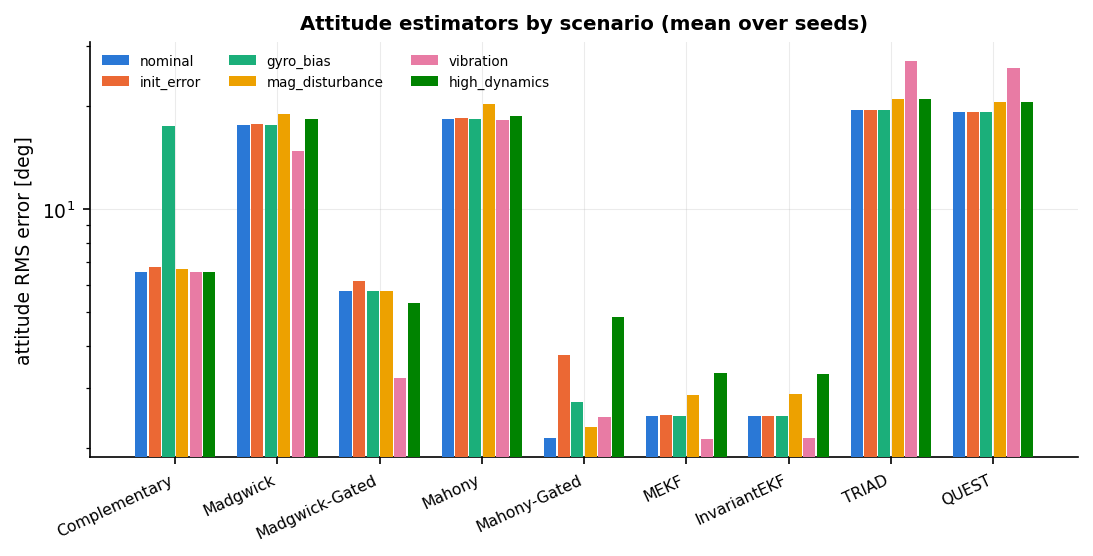
\includegraphics[width=\textwidth]{figures/imu_overview.png}
\caption{RMS attitude error of the nine attitude estimators by scenario (log scale). Three
tiers: the covariance-carrying filters and the gated Mahony filter at \SIrange{2}{5}{\degree}, the
gated Madgwick and the complementary filter at \SIrange{3}{7}{\degree} (\SI{18}{\degree} for the
latter with a gyro bias it cannot estimate), and everything that trusts the accelerometer during
a banked turn at \SIrange{15}{27}{\degree}.}
\label{fig:res-imu}
\end{figure}

\section{The mission decides the ranking}

The table separates into three tiers, and the separation is made by one feature of the flight
rather than by the sophistication of the estimators. In a coordinated turn at \ang{25} of bank
the accelerometer measures the specific force, which points along the body vertical and not
along gravity; an estimator that uses it as a gravity reference tilts its estimate by the bank
angle for the duration of the turn, and the tilt error is amplified into heading error by the
\ang{65} dip of the magnetic field ($\tan I = 2.14$). The three turns occupy a third of the
mission. The published Madgwick and Mahony filters, TRIAD and QUEST all use the accelerometer
without qualification, and all four read \SIrange{17.6}{19.6}{\degree} RMS on the nominal
flight, essentially all of it in yaw (\SIrange{15}{17}{\degree}) with peak errors of
\SIrange{71}{88}{\degree} inside the turns; the benchmark's divergence flag is raised for all of
them. Their nominal, initial-error and gyro-bias columns are identical to two decimals, because
the turn error dominates everything else.

The estimators that recognise the turn form the upper tiers. The MEKF and the invariant EKF
carry a measurement-covariance model that inflates the accelerometer noise with the deviation of
the specific-force magnitude from $g$ and with the rate-driven manoeuvre bound of
\cref{ch:att-mekf}, so the accelerometer is edited out during the turns and the attitude is
coasted on the gyro and the magnetometer; they read \num{2.48} and \SI{2.49}{\degree} on
nominal, of which \SI{2.2}{\degree} is yaw and about \SI{0.65}{\degree} of that is the structural
heading error of the uncompensated hard iron. The gated variants of Mahony and Madgwick apply
the same disturbance weight to the accelerometer term of the published algorithms, and the
gated Mahony filter --- with its integral term estimating the gyro bias --- is the best
estimator of the family on the nominal flight at \SI{2.14}{\degree}, for \SI{132}{\nano\second}
per sample against \SI{2.0}{\micro\second} for the MEKF. The gated Madgwick filter, which has no
bias state, reads \SI{5.8}{\degree}; the fixed-gain complementary filter, which has the gate but
no bias state either, \SI{6.6}{\degree}.

\section{Scenario by scenario}

The \code{gyro\_bias} column is the one on which the bias state pays: the MEKF, IEKF and gated
Mahony filter absorb a \SI{3}{\degree\per\second} bias at no cost (\num{2.48}, \num{2.49} and
\SI{2.74}{\degree}, with an identified bias good to \SIrange{0.2}{0.35}{\degree\per\second}),
while the complementary filter goes from \num{6.6} to \SI{17.6}{\degree} and TRIAD and QUEST,
which do not integrate the gyro at all, are unaffected because they never used it. The
\code{mag\_disturbance} column costs every estimator \SIrange{0.2}{2}{\degree} of heading; the
covariance filters take \SI{0.4}{\degree}, the gated Mahony \SI{0.2}{\degree}, the ungated filters
\SIrange{1.4}{2}{\degree}. \code{vibration}, which adds broadband accelerometer noise, is free
for every filter with a low-pass structure (the covariance filters even improve, to
\SI{2.14}{\degree}, because the higher measured accelerometer variance is what their
measurement model was already assuming) and is the worst scenario for the single-frame
solutions (\num{26}--\SI{27}{\degree}), which have no memory to average it with.
\code{high\_dynamics} adds faster turns; the covariance filters read \SI{3.3}{\degree} and the
gated Mahony filter \SI{4.8}{\degree}, with the difference being the interval during which the
gate has switched the accelerometer out and the heading drifts on the gyro. The \ang{46}
initial error of \code{init\_error} is removed by every estimator with a correction path in
\SIrange{8}{10}{\second}, and the column is otherwise a copy of \code{nominal}.

\section{What the attitude results say}

For a fixed-wing or multirotor airframe that turns, the accelerometer is not a gravity sensor
for a third of the flight, and the estimator must know it. That knowledge can be a full
measurement-covariance model (MEKF, IEKF) or a scalar gate on the accelerometer weight of a
\SI{130}{\nano\second} complementary filter; the benchmark finds no accuracy argument for the
former over the gated Mahony filter on this mission, and a cost argument of fifteen to one for
the latter. The covariance filters keep two advantages that the table does not show: they
report a covariance, which the vehicle's navigation filter needs, and they are within a degree
of their own best on every scenario, which the gated filters are not (\num{2.1}--\SI{4.8}{\degree}
for Mahony-Gated against \num{2.1}--\SI{3.3}{\degree} for the MEKF). The single-frame
solutions are what they were designed to be, an initialisation and a fallback, and should not
be read as estimators. The residual of the best filters, \SI{2}{\degree} of heading, is set by
the compass calibration and not by the estimation algorithm.

The cross-check against the \code{ahrs} reference implementation (\cref{sec:me-crossval}) puts
the library's Madgwick and Mahony filters within \SI{0.0014}{\degree} of the published code on the
same data, so the \SI{18}{\degree} of the ungated filters is the behaviour of the published
algorithms on this mission and not an implementation artefact.
